

\chapter{Introduction} 

\label{Chapter1} 


%----------------------------------------------------------------------------------------
%	GENERAL INTRODUCTION
%----------------------------------------------------------------------------------------

In the last couple of decades, computers  have found a number of applications in biology and medicine. We may even say they have become an essential tool in revealing the questions of life. A significant role in those problems was played by machine learning, a branch of artificial intelligence concerned with the construction of models capable of learning from data . Probably the most inspiring example comes from the field of bioinformatics where scientists have used the methods from  statistics and artificial intelligence to sequence the human genome for the first time. If that was one of the first results, then, what can we expect from the future? \\

Besides the genomic data which is represented as a sequence of nucleotides, a great amount of  biological data can be aquired by different imaging methods such as microscopy, PET or CT imaging and others. That is were the medical imaging and bioimage analysis fields come from. The field of bioimage analysis studies the biological problems by examining an image, or image sequence of a process of interest, while the medical image analysis is concerned with developing of methods that will help in a medical diagnosis process based on imaging. \\

The above mentioned field of medical image analysis overlaps with a field of computer aided diagnosis (CAD) which collects a broader range of methods used as an assistance to the doctors. An application area of this Thesis would fit the best in that field. This thesis will take a direction in a specific task of assistance to an autoimmune disease diagnosis, with a special emphasis to human interpretable models. During the recent few years, this specific problem has been solved very efficiently. If the problem has been solved, why is this thesis taking another look at it? \\

The goal of the Thesis is to provide a  CAD method capable of making a decision based on a microscopic image of HEp-2 cell in a human intepretable way. To demonstrate the importance of intepretable model in CAD systems, I consider the following scenario.

%----------------------------------
%   MOTIVATIONAL SCENARIO
%----------------------------------

\section{Motivational Scenario}

Imagine a following scenario. \textit{Peter} is a doctor, an immunologist. Being an immunologist, his job is to find out which autoimmune disease a patient has. As that is an extremly hard task, Jules uses  computer assistance - an artifical intelligence program named \textit{Hal}. Hal's role is to confirm Peter's diagnosis, or to provide an additional insight if the decision is hard to make. \\

We are interested in the situation where Peter and Hal have made a conflicted decision. There are two cases representing the insight Hal can provide. Each case reflects Hal's interior structure : a \textbf{black-box} model\footnote{By black-box model we assume a model for which we can only observe it's output, not a decision process} or an \textbf{ interpretable} one. If Hal is the black-box model, it is not much of an assistance, as Hal can't elaborate it's decision. We can only agree we disagree. In this case, Hal is not much of a help. \\

On the other hand, if Hal is an interpretable model, it can elaborate it's decision and help Peter. If a wrong decision was made by Hal, Peter can observe it's model parameters, correct the wrong one(s), query again and see if new result supports it's decision. If a wrong decision was made by Peter, Peter can observe Hal's model, find the parameters he might have overseen and correct his diagnosis. \\

The example clearly demonstrates one  thing -- the importance of interpretable models for CAD systems. Computers have proven their ability of inferring from a large amount of data, usually outperforming humans, but in specific situations, a good and accurate model is not enough. We also need to interpret results if we are going to use them.

\section{Detecting the autoimmune diseases}

As mentioned already, this Thesis will address the specific topic of autoimmune diseases classification. The human immune system creates antibodies to fight against infections whereas antinuclear antibodies affect healthy tissues. The Antinuclear Autoantibodies test (ANA) is widely used to determine whether the immune system is developing antibodies or not. Indirect immunofluorescence (IIF ) with HEp-2 cells is the recommended method to diagnose the presence of antinuclear autoantibodies in patient serum. \\

IIF method consists of four consecutive steps:
\begin{itemize}
	\item cell segmentation
 	\item intensity level classification
 	\item mitosis detection
 	\item staining pattern classification
\end{itemize}

The final step usually classifies cell images into one of following patterns: homoge
neous, speckled, nucleolar, cytoplasmic, centromere (see figure \ref{fig:CellExamples}). Some variations may be introduced in different datasets due to large number of possible patterns. Those staining patterns further have a clinical associations with a specific autoimmune disease such as Scleroderma, malignant tumor, Lupus nephritis and others. \\

\begin{figure}[htbp]
	\centering
	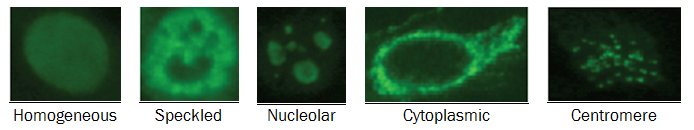
\includegraphics[scale=0.7]{Figures/introduction/cell_examples}
	\rule{35em}{0.5pt}
	\caption[Cell examples]{HEp-2 cell patterns}
	\label{fig:CellExamples}

\end{figure}

Although IIF posses qualities such as high sensitivity and a large number of antigens
that can be detected, it suffers from numerous shortcomings. The most important ones
are liability to subjectivity and time and labour consuming. \\

In order to avoid any kind of subjectivity , there is a great need for standardization and formalization of the mentioned procedure. Addressing this problem calls for CAD techniques which combines methods from machine learning and image analysis.

\section{Problem statement}

The content of the thesis proposes solutions for three major steps in the IFF process. \\

First of all, in order to find out a cell's pattern, cells should be isolated from an image aquired by IFF. As it is going to be explained (see chapter \ref{Chapter3}), although the problem of cell segmentation has been studied for more than 50 years, segmenting HEp-2 cells still suffers from certain problems, mostly due to different green flourescent protein apsorbtion accross the cells. This thesis proposes a method based on a region growing algorithm that demonstrates an encouraging result for overcoming mentioned problems. \\

Once we have isolated the cells, the next step is to determine the fluorescent intensity of an image. The fluorescent intensity level can take three different values, namely \textit{positive}, \textit{intermediate} and \textit{negative}. A negative value means there are no observable cells in an image, while positive marks easily observable cells.  \\

The final step presents a novel approach to the staining pattern classification. The current state of the art solution solves the problem very successfully, but acts like  black-box solutions not providing any explanation for the decision. This thesis tends to develop a method based on the human interpretable representation and reasoning. As IF-THEN rules are the most natural way of representing human knowledge,  the thesis will follow a rule mining approach, such as Inductive Logic Programming (ILP). \\